\documentclass[10pt,a4paper]{article}
\usepackage[utf8]{inputenc}
\usepackage[finnish]{babel}
\usepackage[T1]{fontenc}
\usepackage{graphicx}
\begin{document}

\title{A* ja Dikstra vertailussa}
\author{Matti Nelimarkka}

\setlength{\parindent}{0pt}
\setlength{\parskip}{1ex}

\maketitle

\newpage

\section*{Tehtävänanto}

Toteuta yleinen ohjelma verkon käsittelyä varten, siten että siinä on mahdollisuus säilöä solmuja ja solmujen välisiä kaaria. Verkko tulee voida määritellä ulkoisessa tiedostossa muodossa \texttt{<solmu 1>:<solmu 2>:<etäisyys solmusta 1 solmuun 2>}, esimerkiksi:

\begin{verbatim}
a:b:5
a:c:10
a:d:1
c:b:4
d:c:10
\end{verbatim}

Lisäksi toteuta lyhyimmän polun etsintä sekä Dikstran algoritmilla \cite{dikstra} että A*-algoritmilla \cite{astar}. Vertaa näitä kahta toteutustapaa toisiinsa empiirisesti.

\section{Toteutus}

Ohjelma on toteutettu oliomallinnusta hyödyntäen: paketteja, rajapintoja ja perintäsuhteita on käytetty selkeyttämään ohjelman rakennetta. Ohjelma koostuu neljästä paketista

\begin{description}
\item[datastructures] sisältää ohjelman toiminnan kannalta välttämättömät itse toteutetut tietorakenteet kekoa, hajautustaulua ja listaa varten. Tarkemmin tätä pakettia käsitellään kappaleessa \ref{datastructures}.
\item[model] sisältää ohjelman tarvitsemat itsenäiset toteutustietorakenteet, yleisen muodon verkon sekä erityiset versiot verkosta, jotka toteuttavat tutkittava olevat Dikstran sekä A*-algoritmit. Yleistä verkkoa on esitelty tarkemmin kappaleessa \ref{model.graph} ja lyhyimmän polun etsintää kappaleessa \ref{path}.
\item[io] tarjoaa palveluja tiedoston lukemiseen tekstiformaatista ohjelman ymmärtämäksi verkoksi. Tätä käsitellään kappaleessa \ref{io}.
\item[test] sisältää ohjelman muiden luokkien testaamiseen tarvittavat luokat. Ohjelman jokaiselle luokalle on kirjoitettu yksikkötestit. Testausprosessia on käsitelty tarkemmin kappaleessa \ref{test}.
\end{description}


\subsection{Omat tietorakenteet}
\label{datastructures}

Tietorakenteiden harjoitustyön luonteen vuoksi toteutukseen on kuulunut omien tietorakenteiden kehittäminen ja testaaminen. Käytännöllisistä syistä johtuen tietorakenteeni vastaavat \textbf{java.util}-paketin tietorakenteita, koska tämä mahdollisti ketterämmän kehityksen\footnote{Muuttujat on määritelty yleisten rajapintojen kautta, jolloin niiden implementaatioluokat pystyi helposti vaihtamaan Javan rajapintaa toteuttavasta luokasta omaan toteutukseeni.} ja Javan valmiiden toiminnallisuuksien käytön osana ohjelmaa. Täsmällisesti toteutussuhteet on esitetty taulukossa \ref{omat_tietorakenteet}.

\begin{table}

\begin{tabular}{l|l}
Toteuttava luokka & Rajapinta \\ 
\hline 
\texttt{MyMap} & \texttt{java.util.Map} \\
\texttt{MyHeap} & \texttt{java.util.Queue} \\ 
\texttt{MyList} & \texttt{java.util.List} \\ 
\texttt{MySet} & \texttt{java.util.Set} \\ 
\texttt{MyIterator} & \texttt{java.util.ListIterator} \\ 
\end{tabular} 

\caption{Omien tietorakenteiden vastaavuus Javan tietorakenteiden kanssa}
\label{omat_tietorakenteet}
\end{table}



\subsection{Malli}
\label{model.graph}

\subsection{Lyhyimmän polun etsintä}
\label{path}

\subsection{Tiedosto-operaatiot}
\label{io}

\section{Testaus}
\label{test}

Ohjelman kukin luokka on testattu erikseen JUnit-testein. Arvio code coveragesta...

Lyhyimmän polun etsimiseen tarkoitetussa testissä käytettiin apuna kolmentoista solmun verkkoa, joka on esitetty kuvassa \ref{testiverkko}. Verkko on pääosin symmetrinen, mutta kaari solmusta 12 solmuun 11 on yksisuuntainen. Kaarien painoissa on myös luotu tilanteita, joissa tietoisesti lyhyin reitti vie enemmän askelia -- tällä on tarkoitus testata reitinhakualgoritmin toimintaa.

\begin{figure}
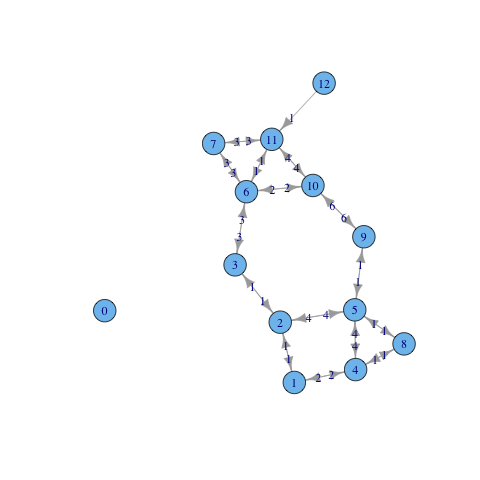
\includegraphics[scale=.5]{test_network.png} 
\caption{Lyhyimmän polun etsimiseen käytetty testiverkko}
\label{testiverkko}
\end{figure}

Täsmällisesti testit toteutettiin seuraaville tapauksille:

\begin{itemize}
\item Solmun 0 etäisyys kaikista muista solmuista tulee olla ääretön.
\item Kaikkien muiden solmujen etäisyys solmusta 0 tulee olla ääretön.
\item Etäisyys solmusta 12 solmuun 11 tulee olla 1.
\item Etäisyys solmusta 11 solmuun 12 tulee olla ääretön.
\item Lyhyin reitti solmusta 1 solmuun 5 kulkee solmujen 4 ja 8 kautta, ja muodostetun reitin pituus on 4.
\item Lyhyin reitti solmusta 5 solmuun 6 kulkee solmujen 2 ja 3 kautta, ja muodostetun reitin pituus on 8.
\item Lyhyin reitti solmusta 1 solmuun 11 kulkee solmujen 2, 3 ja 6 kautta, ja muodostetun reitin pituus on 6.
\item Lyhyin reitti solmusta 4 solmuun 5 kulkee solmun 8 kautta, ja muodostetun reitin pituus on 2.
\end{itemize}

Testit on toteutettu abstraktille yläluokalle \texttt{ShortestPathGraph}, jolloin samaa testikoodia voidaan käyttää sekä luokille \texttt{AStarPathGraph} sekä \texttt{DikstraPathGraph}.

\section{Evaluaatio}

\bibliographystyle{apalike} 
\bibliography{doc}

\end{document}